
\documentclass[journal]{IEEEtran}
%\usepackage{lineno}
%\linenumbers
%\usepackage{cite}

\ifCLASSINFOpdf
  \usepackage[pdftex]{graphicx}
  \graphicspath{pics/}
  \DeclareGraphicsExtensions{.pdf,.jpeg,.png,.jpg}
\else

\fi

\hyphenation{}


\begin{document}
\title{31606 - Assignment number NUMBER}
\author{YOUR GROUP NUMBER, NAMES AND STU-NUMBERS}
%\markboth{Project description}%
%{}


% make the title area
\maketitle

%\IEEEpeerreviewmaketitle

\section{Summary and objectives}
The goal with these reports is to provide a situation where specific tasks need to be solved as a team and where results are documented in a professional and concise way. In addition, the contents of the hands-on will provide you with an idea of where you stand in the course relative to the learning objectives. While it might be hard in the beginning, documentation of results will play an increasing role in your career. Please follow below guidelines when preparing your report.

\subsection{Example text} 
The convolution operation plays an important role in signal processing. Knowing the impulse response of a linear, time-invariant system, the system output can be computed by convolution of an arbitrary input signal with the systems impulse resposne. The convolution theorem translates this operationn to the frequncy domain.
The first part of the report describes the filtering of a delicious chocolate cake through a infinite impulse response (IIR) filter, resulting in another declicious vanilla cake. The second part describes a running beer filter as a prototype for finite impulse response (FIR) filters. The characterization of the filter is described, along with the results of some arbitrary test signals.
The results show that you can also have fun at later stages of your academic career, and that it is actually tough to condense the information to its essentials when you only have 4 pages to fill including pictures.

\section{Methods}
Describe your methods here. Describe how you tackle the problem and why you think it is a good idea to do it exactly this way. Avoid lengthy repetition of the content of the book and restrict yourself to the most essentual information. Provide all the information required to reproduce your results one to one.

The optimal number of bicycles to have is given by eq. \ref{eq:bikes}
\begin{equation}\label{eq:bikes}
 N_b = n + 1 \qquad \mbox{constrained by:} \ \ N_b < s
\end{equation}

where $N_b$ refers to the optimal number of bicycles, $n$ to the number of bicycles you have at the moment, and $s$ the number of bicycles where your spouse will kick you out.


\subsection{Figures}
Prepare your figures such that they fit in width within one column, that the lines are visible and that all fonts are readable. As a guideline, the font size in the figures should be at least the size of the running text. Reduce the number of figures to a minimum. If you have a lot of information, provide panels and label each panel with a capital letter in the top left corner (i.e., A, B, C, ...). Refer to all figures in the running text.  

\subsection{Figure captions}
Please provide figure captions where you describe the main contents of the corresponding figure. This might look as in figure \ref{fig:eyes}:
\begin{figure}
 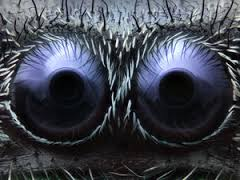
\includegraphics[width=\columnwidth]{eyes}
 \caption{These are eyes of some insect species. There are two of them, located on the left and on the right hand side. They look weird - and they will observe you if you follow the rules.}
 \label{fig:eyes}
\end{figure}


\section{Results}
Describe the results you obtained. Make sure you mention all the correct points and refer to the figures you produced.

\section{Discussion}
Provide some more general comments putting the specific points you found out in the single parts into a bigger context and how they connect to the rest of the conbtants of the course.




\end{document}


